\documentclass[a4paper, 12pt]{book}

\usepackage[utf8]{inputenc}
\usepackage{blindtext}
\usepackage{graphicx}
\usepackage{pgfplotstable}
\usepackage{booktabs}
\usepackage{filecontents}
\usepackage{longtable}
\usepackage{float}
\usepackage[T1]{fontenc}
\usepackage{tocloft}
\usepackage[backend=biber]{biblatex}
\addbibresource{references.bib}
\usepackage[skip=5pt plus1pt, indent=0pt]{parskip}

\usepackage[hidelinks]{hyperref}
\hypersetup{
    linktoc=all
    allcolors=black
}

\graphicspath{
  {./images/}
  {./troubleshooting/}
  {./troubleshooting/crumb-structures/}
  {./history/}
  {./images/external/}
}

\advance\cftsecnumwidth 0.5em\relax
\advance\cftsubsecindent 0.5em\relax
\advance\cftsubsecnumwidth 0.5em\relax
\begin{document}

\begin{titlepage}
	\centering
  \includegraphics[width=\textwidth]{cover-page}
  Version:
  \today
\end{titlepage}


\frontmatter

\tableofcontents

\chapter{Foreword}
Hopefully one day there is going to be an awesome foreword
by another break baker!

\chapter{Preface}
If there is the one food from Germany it is probably bread. There are thousands
of different varieties of bread in Germany. Making bread has been an integral part
of our culture. Beginning my studies in Göttingen for the first time I was faced
with buying bread on my own. In Germany that is no easy task
as the varieties of bread are endless. I started to check the packaging
of different bread types and noticed how there were surprisingly
many ingredients in most of the breads found in a common supermarket.


\chapter{Acknowledgements}
This book would not have been possible without the help of the community. Thank you very much for all the support. \\ \\


\begin{filecontents}{supporters.csv}
  \end{filecontents}

  {\large All supporters sorted by name}

  \pgfplotstableset{
  begin table=\begin{longtable},
  end table=\end{longtable},
  }

  \pgfplotstabletypeset[col sep=comma,
  header=true,
  columns={Name},      % display specified columns
  columns/Name/.style={column type=l,string type},
  % requires booktabs to place horiz rules
  every head row/.style={before row=\toprule, after row=\midrule\endhead},
  every last row/.style={after row=\bottomrule}
  ]{supporters.csv}


\mainmatter

\chapter{The history of sourdough}
Sourdough has been made since ancient times. The exact origins of fermented
bread are, however, unknown. One of the most ancient preserved
sourdough breads has been excavated in Switzerland.
However, based on recent research, some scientists speculate that sourdough
bread had already been made in 12000 BC in ancient Jordan \cite{jordan+bread}.

\includegraphics[width=\textwidth]{einkorn-crumb}

\chapter{How sourdough works}
In this chapter, we will cover the basics of how sourdough ferments.
First, we will look at the enzymatic reactions that take place
in your flour the moment you add water, triggering the fermentation
process. Then, in order to better understand this process, we will
learn more about the yeast and bacterial microorganisms involved.

\begin{figure}[!htb]
  \includegraphics[width=\textwidth]{infographic-enzymes}
  \caption{How amylases and proteases interact with flour}
  \label{infographic-enzymes}
\end{figure}

\section{Enzymatic reactions}

To understand the many enzymatic reactions that take place when flour
and water are mixed, we must first understand seeds and their role in
the lifecycle of wheat and other grains.

Seeds are the primary means by which many plants, including wheat,
reproduce. Each seed contains the embryo of another plant, and must
therefore contain all the nutrients that new plant requires to grow.

When the seed is dry, it is in hibernation mode and can sometimes be
stored for several years. The moment it comes into contact with water,
however, it begins to sprout. The seed turns into a germ, requiring the
stored nutrients to be converted into something the plant can use while
it grows. The catalyst that makes the associated reactions possible is water.

The seed typically contains the first prototypical leaves of the plant,
and can put down roots using the stored nutrients inside. Once those leaves
break through the soil and come into contact with the sunlight above, they
begin to photosynthesize. This process is the plant's engine, and with the
energy photosynthesis produces, the plant can continue to grow more roots,
enabling it to access additional nutrients from the soil. These additional
nutrients allow the plant to grow more leaves, increasing its photosynthetic
activity so that it can thrive in its new environment.

Of course, a ground flour can no longer sprout. But the enzymes that
trigger this process are still present. That's why it's important not to
mill grains at too high a temperature, as doing so could damage some of
these enzymes.

Normally, the grain seed shields the germ against pathogens. However, as the
grain is ground into flour, the contents of the seed are exposed. This is ideal
for our sourdough microorganisms.

Neither the yeast, considered a saprotrophic fungus, nor the bacteria can
prepare their own food. However, as the enzymes are activated, the food they
need becomes available, allowing them to feed and multiply.

The two main enzymes involved in this process are \textbf{amylase} and
\textbf{protease}. For reasons that will soon be clear, they are of the utmost
importance to the home baker, and their role in the making of sourdough is a
key puzzle piece to making better-tasting bread.

\subsection{Amylase}

Sometimes, when you chew on a potato or a piece of bread
for a long period of time, you'll begin to notice a sweet flavor in
your mouth. That's because your salivary glands produce amylase.
Amylase breaks down complex starch molecules into easily-digestible
sugars. The germ needs this to produce more plant matter, and your body
needs this to kick-start the digestive process. Normally, the microorganisms
on the surface of the grain can't consume the freed maltose molecules,
which remain hidden inside the germ. But as we grind the flour, a feeding
frenzy begins. Generally, the warmer the temperature, the faster this
reaction takes place. That's why a long fermentation is key to making
great bread. It takes time for the amylase to break down most of
the starch into simple sugars, which are not only consumed by the
yeast but are also essential to the \it{Maillard reaction}
that's responsible for enhanced browning during the baking process.

If you're a hobby brewer, you'll know that it's important to keep
your beer at certain temperatures to allow the different amylases to
convert the contained starches into sugar \cite{beer+amylase}. This
process is so important that there's a frequently used test to
determine whether or not all the starches have been converted.

This test, called the Iodine Starch Test, involves mixing iodine into
a sample of your brew and checking the color. If it's blue or black,
you know you still have unconverted starches. I wonder if such a test
would also work for bread dough?

Industrial bakers that add especially active yeast to produce bread
in a short amount of time face a similar issue. Their approach is to
add malted flour to the dough. The malted flour contains many enzymes,
and thus speeds up the fermentation process. The next time you're at the
supermarket, check the packaging of the bread you buy. If you find
{\it malt} in the list of ingredients, chances are this strategy was
used.

Note that there are actually two categories of malt. One is
{\it enzymatically active malt}, which has not been heated to above 70°C,
where the amylases start to degrade. The other is {\it inactive malt},
which has been heated to higher temperatures and thus has no impact on
your flour.

\subsection{Protease}

The second very important enzyme is the protease. Proteases
break down proteins into smaller proteins or amino acids.
Gluten for instance is a storage protein built by wheat.
The gluten is broken down and converted the moment the
seed starts to sprout. That's because the seed needs
smaller amino acids to build the roots and other plant material.
If you ever try to make a wheat based dough and just keep
it for several days at room temperature you will notice
how your gluten network starts to break down. The dough
no longer holds together. You can just fully tear it apart.
I have had this happen to me when I was trying to make
doughs directly with dried sourdough starter. The fermentation
speed was so low that it took 3-4 days for the dough
to be ready. The root cause for this issue is the protease.
By adding water to the dough the protease was activated
and started to ready amino acids for the germ in order to be
able to sprout. Another interesting experiment that viusalises
the importance of protease is the following. Try to make a
fast dough within 1-2 hours. Simply use a large quantity
of dry yeast. Your dough will be leavened and increase in size.
Bake your dough and notice the crumb of your baked dough.
You will notice that the crumb is quite dense and not as
fluffy as it could be. That's because the protease enzyme
didn't have enough time to do its job. At the start
when kneading your dough is very elastic. It holds together
very well. Over the course of the fermentation process
your dough will become more extensible \cite{protease+enzyme+bread}.
Some of the gluten bonds start to naturally break
down due to the protease proteolysis. This makes it easier
for your dough to be inflated. That's why a long
fermentation process is important when you want to
achieve very fluffy and open crumbs with your sourdough
bread. Next to using great ingredients, the long and
slow fermentation is one of the main reasons why
Neapolitan pizza tastes so great. The soft and fluffy
edge of the pizza is achieved because of the protease
creating a very extensible easy to inflate dough. Because
the fermentation process is typically longer than 8
hours a flour with a higher gluten content is used. There
is more gluten that can be broken down by the protease.
By using a weaker flour you might end up with a dough
that's already broken down too much and will then tear
when trying to make a pizza pie. Traditionally the pizza
has probably been made with sourdough. In modern times
it is made with yeast as handling a yeast based
dough can be done easier on a larger scale. The dough
stays good for a longer period of time. If you were to use
sourdough you might have a window of 30-90 minutes when
your dough is perfect. Afterwards the dough might
start to deteriorate because of bacteria breaking
down the gluten network too much.

\subsection{Improving enzymatic activity}

As explained previously malt is a common trick used
to speed up enzymatic activity. I personally prefer
to avoid malt in most of my recipes. Instead I use
a trick I observed when making whole wheat doughs.
No matter what I tried I could never achieve baking
a whole wheat bread with the desired crust and crumb
texture I was looking for. My doughs would tend to
overferment relatively quickly. When using a flower
with a similar amount of gluten that didn't contain
bran and other outer parts of the grain my doughs turned
out great. I was utilizing an extended autolyse.
That's a fancy word for just mixing flour and water in
advance and letting that mixture sit. Most recipes
call for it as the help to make a dough that has already
started to break down by enzymes. In general it's a great
idea but at the same time you can just reduce the amount
of leavening agent you use. This way the same biochemical
reactions happen and you don't have to mix your dough
several times. My whole wheat game drastically improved
when I stopped using the autolysis. It makes sense if I
think about it now. The first parts of the seed that
are in contact with water are the outer parts. Water
will slowly enter the center parts of the grain. The
moment the seed starts to sprout it needs to outcompete
other nearby seeds. Furthermore it also directly becomes
exposed to other animals and potential hazardous bacteria
and fungi. To accelerate this process most of the enzymes
of the grain are in the outer parts of the hull. They
are being activated first (source needed). So by just
adding a little bit of whole flour to your dough you 
will improve enzymatic activity of your dough. That's
why most of my plain flour doughs typically contain
at least 10-20 percent whole wheat flour.

\begin{figure}
  \includegraphics[width=\textwidth]{whole-wheat-crumb}
  \caption{A whole wheat sourdough bread}
  \label{whole-wheat-crumb}
\end{figure}


By understanding the 2 key enzymes amylase and protease
you will better be able to understand how to make a
dough to your liking. Would you like a dough a softer
or stiffer crumb? Would you like to achieve a darker crust?
Would you like to reduce the amount of gluten in your
final bread? These are all factors you can influence
by adjusting the speed of fermentation.

\section{Yeast}

Yeasts are single celled microorganisms that are part of
the fungus kingdom. Yeast spores that are hundreds
of million years old have been identified by scientists.
There is a wide variety of species and so far around 1500
different species have been recognized. Yeasts are not creating
a mycelium network like mold does for instance
\cite{molecular+mechanisms+yeast}.

\begin{figure}[!htb]
  \centering
  \includegraphics[width=1.0\textwidth]{saccharomyces-cerevisiae-microscope}
  \caption{Saccharomyces cerevisiae: Brewer's yeast under the microscope}
  \label{saccharomyces-cerevisiae-microscope}
\end{figure}


Yeasts are saprotrophic fungi. This means they are not
producing their own food. They rely on external food sources
which they decompose and break down. For yeasts
carbohydrates and broken down to carbon dioxide and
alcohols. The products of this fermentation process
have been used for thousands of years when making
bread or alcoholic beverages. Yeasts can grow
in both aerobic and anaerobic conditions. When oxygen
is present the yeast almost completely produces
carbon dioxide and water. When no oxygen is present
the yeast starts switches its metabolism. The
yeast starts to produce alcoholic compounds \cite{effects+oxygen+yeast+growth}.
The temperatures at which the yeast grows vary. Some
yeasts such as {\it Leucosporidium frigidum} grows
best at temperatures between -2°C up to 20°C. Other
yeast grows better at higher temperatures. The warmer
it is the faster the yeast's metabolism works. The yeast
that you cultivate in your sourdough starter works best
at the temperatures where the grain was grown and at
the point when it was harvested. So if you are from a 
cooler place and cultivate a sourdough starter from
a nordic rye variety, then chances are your yeast
prefers this colder environment. As an example
beer makers discovered that a beneficial yeast lives
in the cold caves around the city of Pilsen, Czech Republic.
This yeast has produced excellent tasting beers at
lower temperatures. Varieties of these strains
are now used to make popular lager beers.

Yeasts in general are very common in the environment.
They can be found on cereal grains, fruits, other plants
in the soil and also in your gut. Very little is known
about the ecology of why yeasts we use for baking
are cultivating the leaves of the plants. The plants
are protected via the cell walls and hardly any
fungi and other bacteria can penetrate. Some fungi and
bacteria are producing enzymes that are able
to break down the cell walls and infect the plant.
There are fungi and bacteria that live within the plant
without causing any distress. These are known as {\it endophytes}.
They are not damaging the plant per se. In fact they are
living in a symbiotic relationship with the host. They
help the plant to protect itself from additional pathogens
that might enter through the leaves of the plant. They
help with water stress, heat stress and nutrient availability. 
In exchange for the service they receive carbon for energy
from the plant host. They are not always strictly mutualistic though.
Sometimes under stress conditions they can become pathogens
on their own \cite{endophytes+in+plants} and decay begin
decaying the plant.

The yeasts we use for baking are
living as as epiphytes on the plant. Compared to
the previously mentioned endophytes they are not
breaching the walls of the cells. Most of them
receive nutrients from rain water, the air or other animals.
These sources also include honeydew produced
by aphids. Pollen that lands on the leaf's surface
is an additional source of food. Interestingly
though when you remove that external food source,
you still find a large variety of epiphytic fungi
and bacteria on the plant's surface. The food
for them is coming directly from the plant it seems.
Some research has shown that the plants are
on purpose releasing some compounds such as sugars,
organic acids, amino acids, some methanol and various
salts via the surface. These nutrients would
then attract the epiphytes to live on the surface.
The plants benefit from enhanced protection against
mold and other pathogens. It is in the best interest
of the epiphytes to keep the plants alive
as long as possible \cite{leaf+surface+sugars+epiphytes}.
More and more research is conducted on using yeasts
as a biocontrol agents to protect plants. These bio-agents
would be food-safe as yeasts are generally considered save.
The yeasts would start to grow on the leaves on the plant
and essentially shield the plants from other molds. This
could be a game changer for wineyeards suffering from mildew.
This could also be helpful to shield the plant against the
psychoactive ergot fungus. The ergot fungus likes to grow
in more humid colder environments and poses a huge
problem to rye farmers. The fungus parasites the plant
and infects it. Consumption of ergot is not recommended
as it is highly toxic to the liver. That's why lawmakers
have recently reduced the amount of allowed ergot contamination
in rye flour. Another interesting experiment from Italian scientists
visualized how important yeasts could be when protecting
plants. They added tiny incisions into some of the grapes.
They would then infect some of the damaged surfaces with
mold. The other wounds they infected with some of the 150
different wild yeast strains isolated from the leaves plus
the mold. When mixing the mold with the yeast the grape
sustained no significant damage \cite{yeasts+biocontrol+agent}.
In another experiment however scientists have shown
how the brewer's yeast became an aggressive pathogen to wine plants.
Initially the yeast lived in symbiosis with the plant. After the grapevine
sustained damages the yeast became opportunistic and started to
attack the plant event producing hyphae to deeply
penetrate the plants tissue.

\section{Bacteria}

\chapter{Making a sourdough starter}
In this chapter you will learn how to make your
own sourdough starter. Before doing so you will
quickly learn about baker's math. Don't worry,
it's a very simple way how to write a recipe which
is cleaner and more scalable.  Once you get the hang
of it you will want to write every recipe this way.
You will learn to understand the signs to determine
your starter's readiness.  Furthermore you will
also learn how to prepare your starter for long-term storage.

\section{Baker's math}
\label{section:bakers-math}

In a large bakery, a determining factor is how
much flour you have at hand. Based on the amount
of flour you have, you can calculate how many
loaves or buns you can make. To make it easy
for bakers, the quantity of each ingredient
is calculated as a percentage based on how much flour you have.
Let me demonstrate this with a small example from
a pizzeria.  In the morning you check and you realize you
have around 1 kilogram of flour.
Your default recipe calls for around 600 grams of water.
That would be a typical pizza dough, not too dry but
also not too wet. Then you would be using around 20 grams
of salt and around 100 grams of sourdough starter.
\footnote{This is my go to pizza dough recipe. In Napoli
modern pizzerias would use fresh or dry yeast. However
traditionally pizza has always been made with sourdough.}
The next day you suddenly have 1.4 kilograms of flour
at hand and thus can make more pizza dough. What do you do?
Do you multiply all the ingredients by 1.4? Yes you could,
but there is an easier way. This is where baker's math
comes in handy. Let's look at the default recipe with baker's
math and then adjust it for the 1.4 kilogram flour quantity.

\begin{figure}[!htb]
  \includegraphics{tables/table-bakers-math-example.pdf}
  \caption{An example table demonstrating how to properly calculate using baker's math}
\end{figure}

Note how each of the ingredients is calculated as a percentage
based on the flour.  The 100 percent is the baseline and represents the absolute
amount of flour that you have at hand. In this case that's 1000 grams
(1 kilogram).

Now let's go back to our example and adjust the flour, as we have
more flour available the next day. As mentioned the next day
we have 1.4 kilograms at hand (1400 grams).

\begin{figure}[H]
  \includegraphics{tables/table-recipe-bakers-math.pdf}
  \caption{An example recipe that uses 1400 grams as its baseline and
  is then calculated using baker's math}
\end{figure}

For each ingredient we calculate the percentage
based on the flour available (1400 grams). So for the water
we calculate 60 percent based on 1400. Open up your
calculator and type in 1400 * 0.6 and you have
the absolute value in grams that you should be using.
For the second day, that is 840 grams. Proceed to do the same
thing for all the other ingredients and you will know
your recipe.


Let's say you would want to use 50 kilograms of flour
the next day. What would you do? You would simply proceed
to calculate the percentages one more time. I like this
way of writing recipes a lot. Imagine you wanted to make
some pasta. You would like to know how much sauce you should
be making. Now rather than making a recipe just for you, a
hungry family arrives. You are tasked with making pasta
for 20 people. How would you calculate the amount of sauce
you need? You go to the internet and check a recipe and then
are completely lost when trying to scale it up.

\section{The process of making a starter}

\begin{figure}[!htb]
  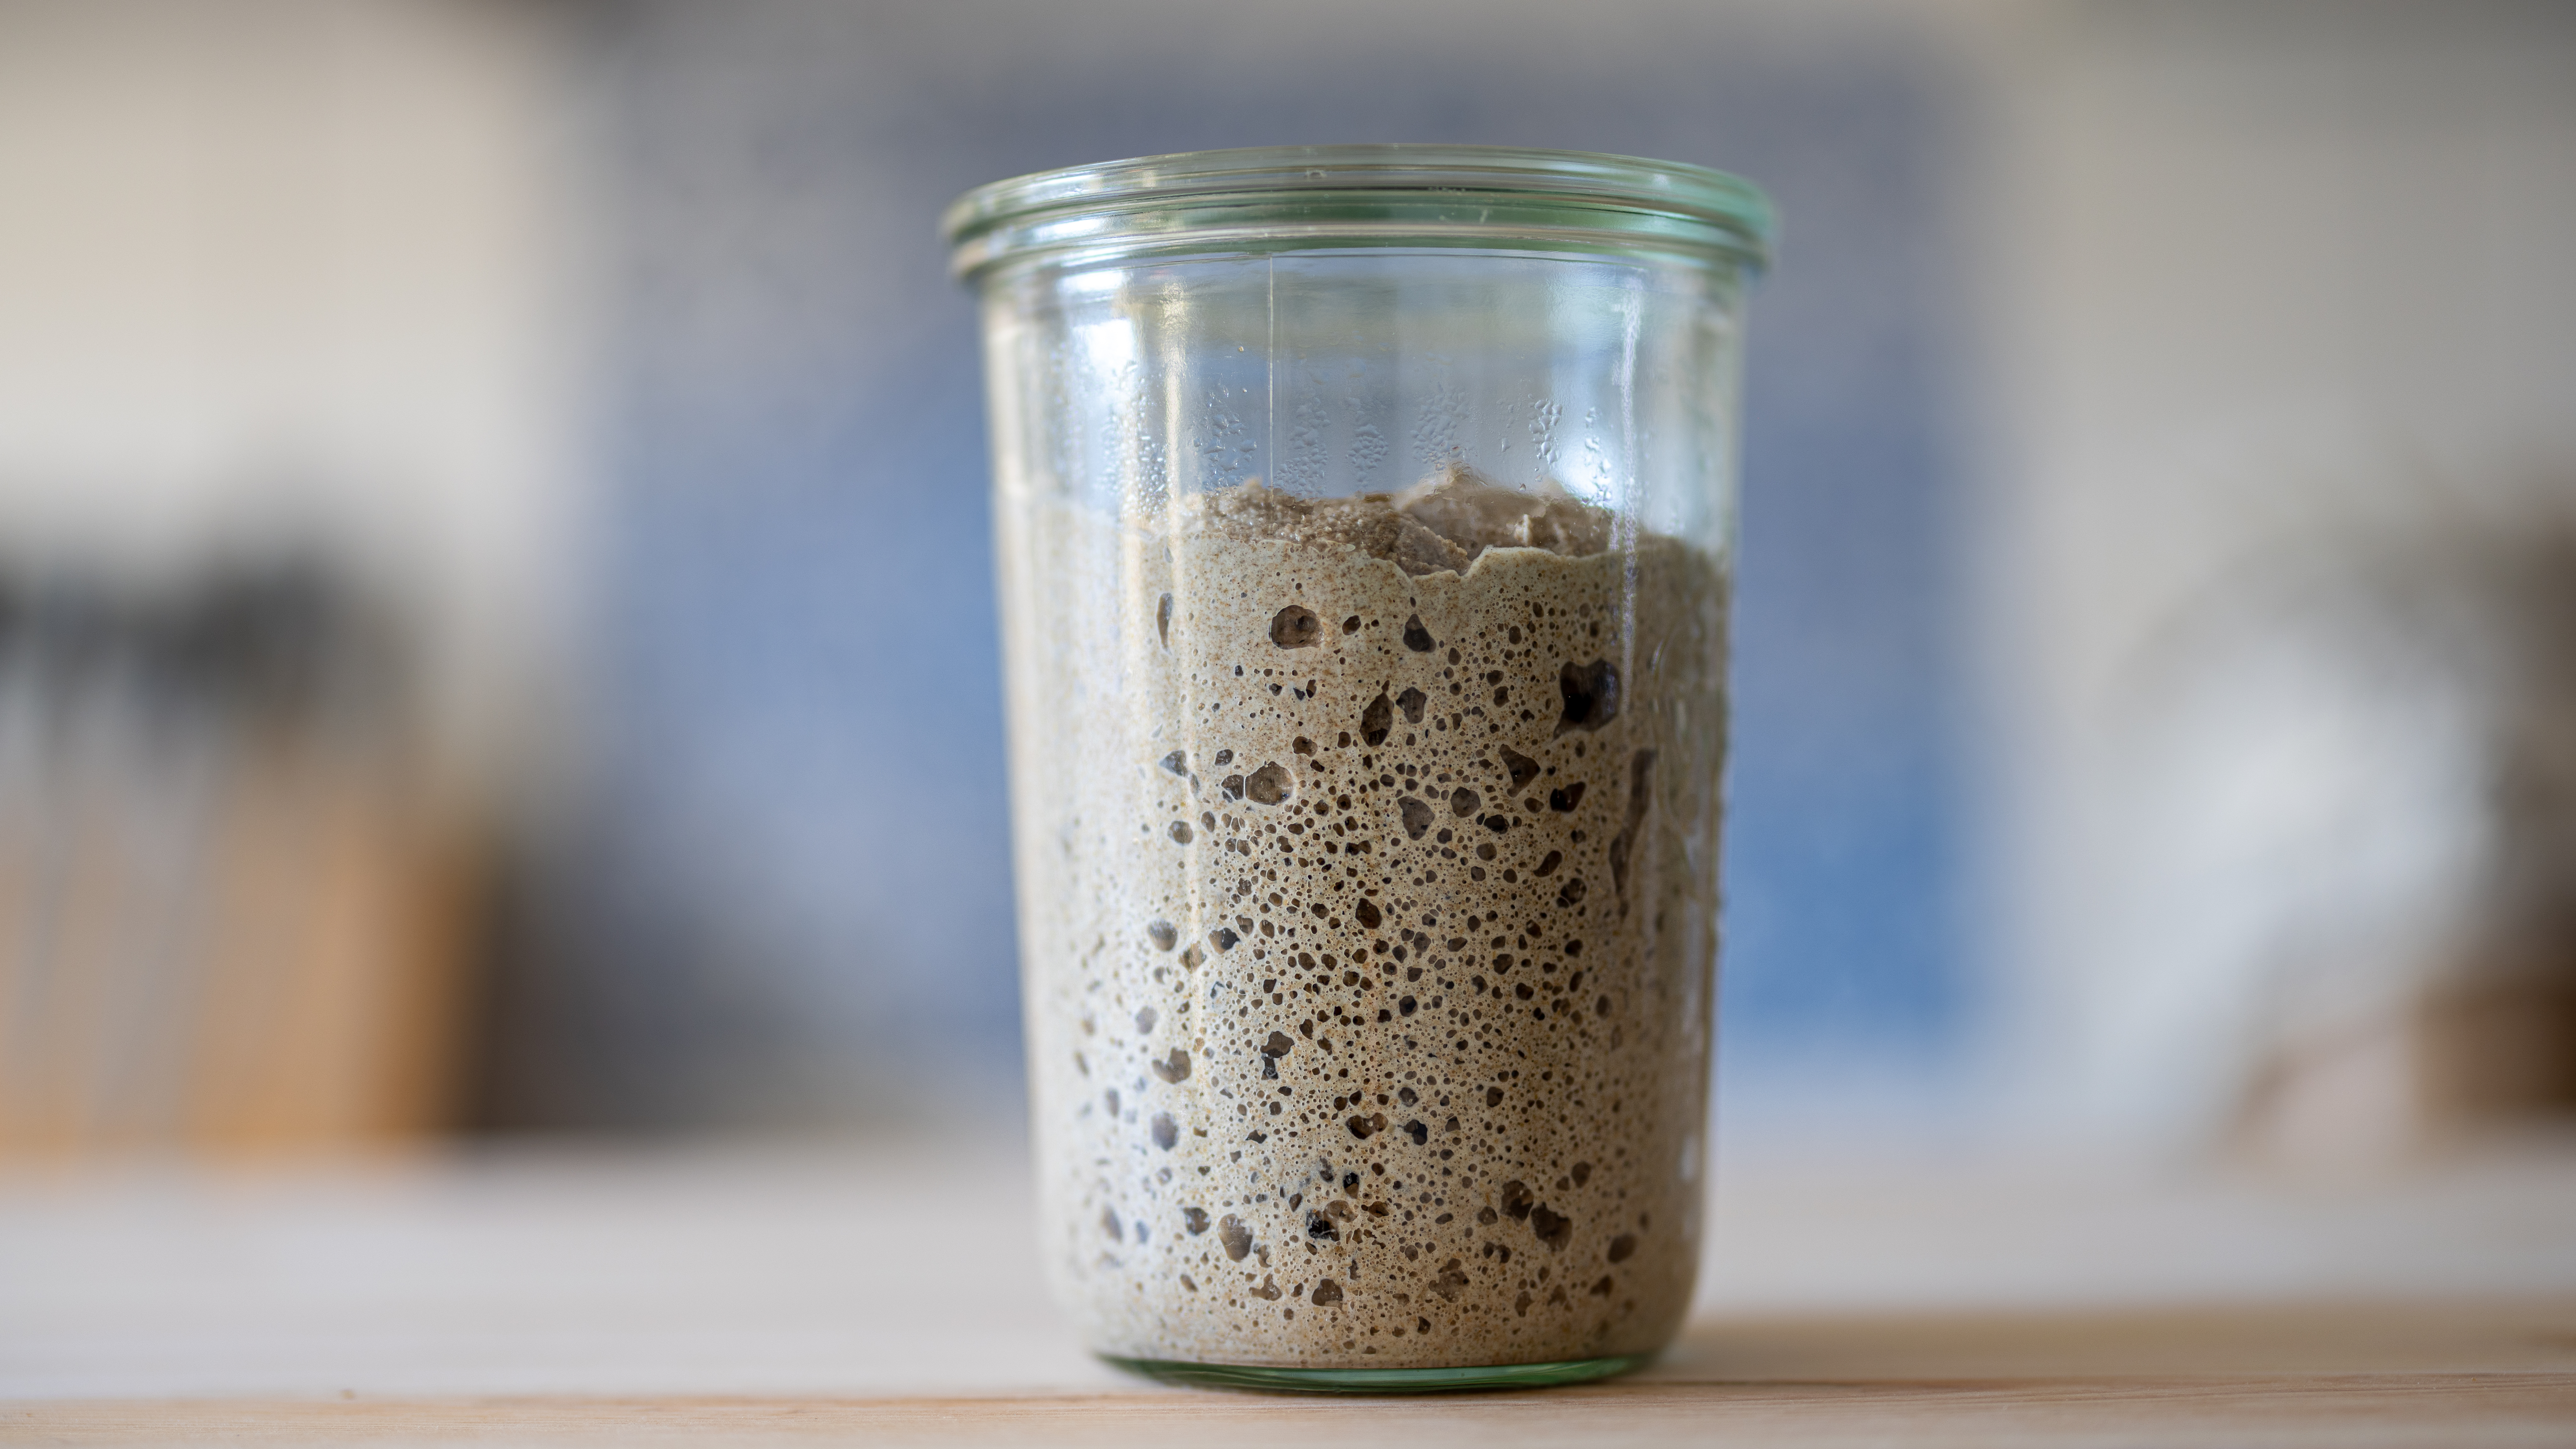
\includegraphics[width=\textwidth]{sourdough-starter.jpg}
  \caption{A very active sourdough starter shown by the bubbles in the dough}
  \label{fig:sourdough-starter}
\end{figure}

Making a sourdough starter is very easy. All you need
is a little bit of patience. The flour you should
use to setup your starter is ideally a whole flour.
You could use whole wheat, whole rye, whole spelt or
any other flour you have. In fact gluten free flours such
as rice or corn would also work. Don't worry, you can
change the flour later. Use whatever whole flour you
already have at hand.

Your flour is contaminated with millions of microbes. As explained
before in the chapter about wild yeast and bacteria, these
microbes live on the surface of the plant. That's why
a whole flour works better because you have more natural
contamination of the microbes you are trying to cultivate
in your starter. More of them live on the hull compared to the
endophytes living in the grain.

Simply weigh around 50 grams of flour and add another 50
grams of water. It doesn't have to be exactly 50 grams of both
water or flour. You could also use less and/or simply eyeball it.
The values are just shown as a reference. Don't use chlorinated
water to setup your starter. It should be bottled water ideally,
or here in Germany we can just use our tap water. Chlorine
is added to water to kill microorganisms. You will not
be able to grow a starter with chlorinated water. The hydration
of your dough is 100 percent. This means you have equal parts
of flour and water. Stir everything together so that all the flour
is properly hydrated. By adding water many of your microbes'
spores become activated. They exit hibernation mode and
become alive again. Cover your mixture with a lid. I like to
use a glass and place another inverted one on top. The container shouldn't
be airtight. You still want some gas exchange to be possible.

\begin{figure}[!htb]
  \includegraphics{figures/fig-starter-process.pdf}
  \caption{The process of making a sourdough starter from scratch}
  \label{fig:sourdough-starter-process}
\end{figure}

Now an epic battle begins. In one study scientists
have identified more than 150 different yeast species living
on a single leaf of a plant \cite{yeasts+biocontrol+agent}.
All of the different yeasts and bacteria are trying to get
the upper hand in this battle. Other pathogens such as mold
are also being activated as we added water. Only the strongest
most adaptable microorganisms will survive. By adding water to the
flour the starches start to degrade. The seedling tries to
sprout but it no longer can. Essential for this process is the
amylase enzyme. The compact starch is broken down to more
digestible sugars to fuel plant growth. Glucose is what the
plant needs in order to grow. The microorganisms that survive
this frenzy are adapted to consuming glucose. Luckily for us
bakers, the yeast and bacteria know very well how to metabolize
glucose. This is what they have been fed in the wild by the plants.
By forming patches on the leaf and protecting the plant from
pathogens they received glucose in return for their services.
Each of the microbes tries to defeat the other by consuming the
food fastest, producing agents to inhibit food uptake by others or by producing
bactericides and/or fungicides. This early stage of the starter
is very interesting as more research could possibly reveal
new fungicides or antibiotics. Depending on where your flour
is from, the starting microbes of your starter might be different
than the ones from another starter. Some people have also reported
how the microbes from your hand or air can influence your starter's
microorganisms. This makes sense to a certain extent. Your
hand's microbes might be good at fermenting your sweat, but
probably not so good and metabolizing glucose. The contamination
of your hands or air might play a minor role in the initial epic
battle. But only the fittest microbes fitting the sourdough's
niche are going to survive. This means the microorganisms that know
how to convert maltose or glucose will have the upper hand. Or the
microbes that ferment the waste of the other microbes. Ethanol created
by the yeast is metabolized by the bacteria in your sourdough. That's
why a sourdough has no alcohol. I can confirm the role of aerial
contamination to a certain extent. When setting up a new sourdough
starter the whole process is quite quick for me. After a few
days my new starter seems to be quite alive already. This might
be due to previous contamination of flour fermenting microbes in
my kitchen.

\begin{figure}[!htb]
  \includegraphics[width=\textwidth]{sourdough-starter-microbial-war}
  \caption{A simple visualization of the microbial warfare that happens during the making of a sourdough starter. The
  wild spores on the plant and flour become activated the moment flour and water is mixed.
  Only the most adapted flour-fermenting microbes will survive. Because of unwanted microbial fermentation it is advised
  to discard the feeding-leftovers of the first days. The surviving yeast and bacteria continuously try to
  outcompete each other for resources. New microbes have a hard time entering the starter and are eliminated.
  }
  \label{fig:sourdough-starter-microbial-war}
\end{figure}


Wait for around 24 hours and observe what happens to your starter.
You might see some early signs of fermentation already. Use your nose
to smell the dough. Look for bubbles in the dough. Your dough
might already have increased in size a little bit. Whatever
you see and notice is a sign of the first battle. Some microbes
have already been outperformed. Others have won the first battle.
After around 24 hours most of the starch has been broken down
and your microbes are hungry for additional sugars. With a spoon
take around 10 grams from the previous day's mixture and place
it in a new container. Again - you could also simply eye ball
all the quantities. It does not matter that much. Mix the 10
grams from the previous day with another 50 grams of flour
and 50 grams of water. Note the ratio of 1:5. I very often use
1 part of old culture with 5 parts of flour and 5 parts of water.
This is also very often the same ratio I use when making a dough.
A dough is nothing else than a sourdough starter with slightly different
properties. I'd always be using around 100-200 grams of starter
for around 1000 grams of flour (baker's math: 10-20 percent).
Homogenize your new mixture again with a spoon. Then cover
the mix again with a glass or a lid. If you notice the top of
your mixture dries out a lot consider using another cover. The
dried-out parts will be composted by more adapted microbes such as
mold. In many user reports, I saw mold being able to damage
the starter when the starter itself dried out a lot. You will
still have some mixture left from your first day. As this contains
possibly dangerous pathogens that have been activated we will discard
this mixture. Once your sourdough starter is mature never
discard it. It's long-fermented flour that is an excellent addon
used to make crackers, pancakes and or delicious hearty sandwich
bread. I also frequently dry it and use it as a rolling agent
for pizzas that I am making.

You should hopefully again see some bubbles, the starter increasing
in size and/or the starter changing its smell. Some people give
up after the second or third day. That is because the signs might no longer
be as dominant as they were on day one. The reason for this lies in only a few
select microbes starting to take over the whole sourdough starter. The most
adaptable ones are going to win. They are very small in quantity and will
grow in population with each subsequent feeding. Even if you see no signs
of activity directly, don't worry. There is activity in
your starter on a microscopic level.

24 hours later again we will repeat the same thing again until
we see that our sourdough starter is active. More on that in the
next section of this book.

\section{Determining starter readiness}

For some people the whole process of setting up a starter takes
only 4 days. For others it can take 7 days, for some even 20 days.
This depends on several factors including how good your wild microbes
are at fermenting flour. Generally speaking, with each feeding
your starter becomes more adapted to its environment. Your
starter will become better at fermenting flour. That's why
a very old and mature starter you receive from a friend might
be stronger than your own starter initially. Over time
your sourdough starter will catch up. Similarly, modern baking
yeast has been isolated like this from century old sourdough
starters.

\begin{figure}[!htb]
  \includegraphics{figures/fig-starter-readiness.pdf}
  \caption{A flow chart showing you how to determine if your sourdough starter is ready to be used.
  For checking readiness look at a size increase and take note of your starter's smell. Both are important
  indicators to check for readiness.}
  \label{fig:sourdough-starter-readiness}
\end{figure}

The key signs to look at are bubbles that you see in your starter
jar. This is a sign that the yeast is metabolizing your
dough and creates \ch{CO2}. The \ch{CO2} is trapped in your dough
matrix and then visualized on the edges of the container.
Also note the size increase of your dough. The amount the dough increases
in size is irrelevant. Some bakers claim it doubles, triples or quadruples.
The amount of size increase depends on your microbes, but also on
the flour that you use to make the starter. Wheat flour contains
more gluten and will thus result in a larger size increase. At
the same time the microbes are probably not more active compared
to when living in rye sourdough. You could only argue that
wheat microbes might be better at breaking down gluten compared
to rye microbes. That's one of the reasons why I decided to change
the flour of my sourdough starter quite often. I had hoped to create
an all-around starter that can ferment all sorts of different flour.\footnote
{Whether this is working I can't scientifically say.
Typically the microbes that have once taken place are very strong
and won't allow other microbes to enter. My starter has initially
been made with rye flour. So chances are that the majority of
my microorganisms are from a rye source.} Your nose is also
a great tool to determine starter readiness. Depending on
your starter's microbiome you should notice either the smell
of lactic acid or acetic acid. Lactic acid has dairy yogurty notes.
The acetic acid has very strong pungent vinegary notes. Some
describe the smell as glue or acetone. Combining the visual clues
of size increase and pockets plus the smell is the best way
to determine starter readiness.

In rare events your flour might be treated and prevent microbe growth.
This can happen if the flour is not organic and a lot of biochemical
agents have been used by the farmer. In that case simply try again
with different flour. 7 days is a good period of time to wait before
trying again.

Another methodology used by some bakers is the so called \emph{float test}.
The idea is to take a piece of your sourdough starter and place it
on top of some water. If the dough is full with gas it will float
on top of the water. If it's not ready, it can't float and will
sink to the bottom. This test does not work with every flour.
Rye flour for instance can't retain the gas as well as wheat flour
and thus in some cases will not float. That's why I personally
don't use this test and can't recommend it.

Once you see your starter is ready I would recommend giving it
one last feeding and then you are ready to make your dough in the
evening or the next day. For the instructions to make your
first dough please refer to the next chapters in this book.

If your first bread failed, chances are your fermentation hasn't
worked as expected. In many cases the source is your sourdough starter. Maybe
the balance of bacteria and yeast isn't optimal yet. In that case a good
solution is to keep feeding your starter once per day. With each feeding your
starter becomes better at fermenting flour. The microbes will adapt more and
more to the environment. Please also consider reading the stiff sourdough starter
chapter in this book. The stiff sourdough starter helps to boost the
yeast part of your sourdough and balance the fermentation.

\section{Maintenance}

\begin{figure}[!htb]
  \includegraphics{figures/fig-starter-maintenance.pdf}
  \caption{A full flowchart showing you how to conduct proper sourdough starter maintenance. You can use a
  piece of your dough as the next starter. You can also use left-over starter and feed it again. Choose an
  option that works best for your own schedule. The chart assumes that you are using a starter at a 100 percent
  hydration level. Adjust the water content accordingly when you use a stiff starter.}
  \label{fig:sourdough-maintenance-process}
\end{figure}

You have made your sourdough starter and your first bread. How do you perform
maintenance for your starter? There are countless of different maintenance
methods out there. Some people go completely crazy about their starter and
perform daily feedings of the starter. The key to understanding how to properly
conduct maintenance is to understand what happens to your starter after you
used it to make a dough. Whatever starter you have left, or a tiny piece of
your bread dough can serve to make your next starter.\footnote{I very often use all my
starter to make a dough. So if the recipe calls for 50g of starter I make
exactly 50g starter in advance. This means I have no starter left. In that
case I would proceed to take tiny bit of the dough at the end of the
fermentation period. This piece I would use to regrow my starter again.}


As explained earlier your starter is adapted
to fermenting flour. The microbes in your starter are very resilient. They
block external pathogens and other microbes. That is the reason why, when
buying a sourdough starter, you will preserve the original microbes. It is
likely that they are not going to change in your starter. They are outcompeting other
microbes when it comes to fermenting flour. Normally everything in nature
starts to decompose after a while. However, the microbes of your starter have
very strong defense mechanisms. In the end, your sourdough starter can be
compared to pickled food. Pickled food has been shown to stay good for a very
long period of time \cite{pickled+foods+expiration}. The acidity of your sourdough starter is quite
toxic to other microbes. The yeast and bacteria though have adapted to living
in the high-acid environment. Compare this to your stomach, the acidity
neutralizes many possible pathogens. As long as your starter has sufficient
food available it will outcompete other microbes. When the starter runs out of
food the microbes will start to sporulate. They prepare for a period of no
food and will then reactivate the moment new food is present. The
spores are very resilient and can survive under extreme conditions.
Scientists have claimed they found 250 million-year-old spores that are still
active \cite{old+spores}. While being spores
they are however more vulnerable to external pathogens such as mold.
Under ideal conditions though the spores can survive for a
long time.

But as long as they stay in the environment of your starter they live
in a very protected environment. Other fungi and bacteria have a hard time decomposing your left over starter mass.
I have seen only very few cases where the starter actually died. It is almost impossible
to kill a starter.

What happens though is that the balance of yeast and
bacteria changes in your starter. The bacteria is more fitted to living
in an acidic environment. This is a problem when you make another dough.
You want to have the proper balance of fluffiness and sour notes.
When a starter has hibernated for a long period, chances are that
you do not have a desirable balance of microbes.
Furthermore, depending on the time your starter hibernated you might only have
sporulated microbes left. So a couple of feedings will help to get your
sourdough starter into the right shape again.

The following are a couple of scenarios that will help you to conduct proper
starter maintenance, depending on when you want to bake the next time.

\textbf{I would like to bake again the next day:}

Simply take whatever starter you have left and feed it again. If you depleted
all your starter you can cut a piece of your dough. The dough itself is
nothing different than a gigantic starter. I recommend a 1:5:5 ratio like
mentioned before. So take 1 piece of starter, feed with 5 parts of flour and 5
parts of water. If it is very hot where you live, or if you want to make the
bread around 24 hours later after your last feeding, change the ratio. In that
case I would go for a 1:10:10 ratio. Sometimes I don't have enough starter.
Then I even use a ratio of 1:50:50 or 1:100:100. Depending on how much new
flour you feed it takes longer for your starter to be ready again.

\textbf{I would like to take a break and bake next week:}

Simply take your leftover starter and place it inside of your fridge. It will stay good
for a very long period. The only thing I see happening is the surface
drying out in the fridge. So I recommend drowning the starter in a little bit
of water. This extra layer of water provides good protection from the top
part drying out. As mold is aerobic it can not grow efficiently under
water \cite{mold+anaerobic}. Before using the starter again simply either stir
the liquid into the dough or drain it. If you drain the liquid you can use it
to make a lacto fermented hot sauce for instance.

The colder it is the longer you preserve a good balance of yeast and
bacteria. Generally, the warmer it is the faster the fermentation process is,
and the colder it is the slower the whole process becomes.
Below 4°C the starter fermentation almost completely stops. The
fermentation speed at low temperatures depends on the
strains of wild yeast and bacteria
that you have cultivated.

\textbf{I would like to take a several months break:}

Drying your starter might be the best option to preserve it in this case. As
you remove humidity and food your microbes will sporulate. As there is no
humidity the spores can resist other pathogens very well. A dried starter can
be good for years.

Simply take your starter and mix it with flour. Try to crumble the starter as
much as possible. Add more flour continuously until you notice that there is no
moisture left. Place the flour starter in a dry place in your house. Let it
dry out even more. If you have a dehydrator you can use this to speed up the
process. Set it to around 30°C and dry the starter for 12-20 hours. The next
day your starter has dried out a bit. It is in a vulnerable state as there is still a bit
of humidity left. Add some more flour to speed up the drying process. Repeat
for another 2 days until you feel that there is no humidity left. This is
important or else it might start to grow mold. Once this is done simply store the
starter in an airtight container. Or you can proceed and freeze
the dried starter. Both options work perfectly fine. Your sporulated starter
is now waiting for your next feeding. If available you can add some silica
bags to the container to further absorb excess moisture.

Initially, it would take 3 days or so for my starter to become alive again
after drying and reactivating it. If I do the same thing now my starter is
sometimes ready after a single feeding. It seems that the microbes adapt. The ones
that survive this shock become dominant subsequently.

So in conclusion the maintenance mode you choose depends on when you want to bake next.
The goal of each new feeding is to make sure your starter
has a desired balance of yeast and bacteria when making a dough. There is no need to provide your
starter with daily feedings, unless it is not mature yet. In that case, each
subsequent feeding will help to make your starter more adept at fermenting
flour.


\chapter{Sourdough starter types}
\section{The regular starter}
\section{Stiff starter}
\section{Liquid starter}
\section{Lievito madre}

\chapter{Flour types}
\section{Wheat like}
\section{Non gluten binding}
\section{Gluten free}
\section{Blending flours}

\chapter{Bread types}
\section{Wheat bread basics}
\section{Non wheat bread basics}
\section{The simplest way to make bread}

\chapter{Wheat sourdough}
\section{The process}
\section{Readying your starter}
\section{Ingredients}
\section{Hydration}
\section{Autolyse}
\section{Fermentolyse}
\section{Dough strength}
\section{Controlling fermentation}
\section{Optional Preshaping}
\section{Shaping}
\section{Proofing}

\chapter{Non wheat bread basics}
\section{Ingredients}
\section{Managing acidity}
\section{To shape or not to shape}
\section{Proofing}

\chapter{Baking}
\section{The role of steam}
\section{Temperature}
\section{Home oven setup}
\section{Dutch ovens}

\chapter{Storing bread}
\section{Fridge}
\section{Room temperature}
\section{Frozen}

\chapter{Troubleshooting}

\section{Debugging your crumb structure}%
\label{section:debugging-crumb-structure}

The crumb structure of your bread provides insights into how well
your fermentation process has gone. You can also spot common flaws
arising from improper technique. This chapter will provide you with information
that you can use to debug your baking process.

\begin{figure}
  \includegraphics[width=\textwidth]{crumb-structures-book}
  \caption[Debugging your crumb structure]{A schematic visualization of
      different crumb structures and their respective causes. The final bread's
      crumb is a key aspect to identify potential issues related to
      fermentation or baking technique.}%
  \label{fig:crumb-structures-book}
\end{figure}

\subsection{Perfect fermentation}

\begin{figure}
  \includegraphics[width=\textwidth]{open-crumb}
  \caption[Perfectly fermented bread]{The bread has a somewhat open crumb
      with areas featuring a honeycomb structure.}%
  \label{fig:open-crumb}
\end{figure}

Of course the perfect fermentation is debatable and highly subjective. To
me the perfect sourdough bread features a crisp crust paired with a fluffy,
somewhat open crumb. This is the perfect balance of different consistencies
when you take a bite.

Some people are chasers of a very open crumb, meaning you have large pockets
of air (alveoli). It's subjective whether that's the style of bread that you like;
however, to achieve it you need to ferment your bread dough perfectly.
It takes a lot of skill both in terms of mastering fermentation and technique
to achieve a crumb structure like that.

Personally, I~like a bread like that, just with a slightly less wild crumb.
The style of crumb I~like is called the \emph{honeycomb crumb}. It's not too open, but
just enough open to make the bread very fluffy. To achieve the previously mentioned open crumb, you
have to touch your dough as little as possible. The more you interact with your
dough, the more you are degassing your dough. Excess touching of the dough
results in the dough's alveoli merging together. The crumb will not be as open.
That's why achieving such a crumb works best if you only ferment
one loaf at a time. Normally, if you have to pre-shape your dough,
you will automatically degas your dough a little bit during the rounding process.
If you skip this step and directly shape your dough, you will achieve a more open crumb.
A good rule of thumb is to not touch your dough for at least 1--2~hours before shaping,
to achieve as open a crumb as possible.

\begin{figure}
  \includegraphics[width=\textwidth]{honeycomb}
  \caption[Honeycomb crumb structure]{A whole-wheat sourdough with an almost
      exclusive honeycomb crumb structure.}%
  \label{fig:honeycomb}
\end{figure}


Now this is problematic when you want to
make multiple loaves at the same time. Pre-shaping is essential as you are required
to divide your large bulk dough into smaller chunks. Without the pre-shaping
process, you would end up with many non-uniform bread doughs. This technique is
also used when making ciabattas. They are typically not shaped. You only cut the
bulk dough into smaller pieces, trying to work the dough as little as possible.
With pre-shaping you will converge your dough's alveoli into more of a honeycomb structure,
as large pockets of air will slightly merge. Similarly to the open crumb structure,
you also have to nail the fermentation process perfectly to achieve this crumb.
Too long a fermentation will result in gas leaking out of your dough while baking.
The honeycombs won't be able to retain the gas. If you ferment for too short a time,
there is not enough gas to inflate the structures. To me this is the perfect
style of crumb. As someone who appreciates jam, no jam will fall through a slice
of this bread compared to an open crumb.

\subsection{Overfermented}%
\label{subsec:overfermented-dough}

\begin{figure}
  \includegraphics[width=\textwidth]{fermented-too-long}
  \caption[Overfermented sourdough bread]{A relatively flat dough that has many tiny pockets of air.}%
  \label{fig:fermented-too-long}
\end{figure}

When fermenting your dough for too long, the protease enzyme starts to
break down the gluten of your flour. Furthermore, the bacteria consume the gluten
in a process called \emph{proteolysis}~\cite{raffaella+di+cagno}.
Bakers also refer to this process as \emph{gluten rot}.
The gluten that normally traps the \ch{CO2} created
by the fermentation process of your microorganisms can no longer keep the
gas inside of the dough. The gas disperses outward resulting in smaller alveoli in your crumb.
The bread itself tends to be very flat in the oven. Bakers often refer
to this style of bread as a \emph{pancake}. The oven spring can be compared
to bread doughs made out of low-gluten flour like einkorn.

Your bread will feature a lot of acidity, a really strong distinctive tang. From
a taste perspective, it might be a little bit too sour. From my own tests with family and
friends (n=15--20), I~can say that this style of bread is typically
appreciated less. However, I~personally really like the hearty strong taste.
It is excellent in combination with something
sweet or a soup.  From a consistency perspective, it is no longer as fluffy as it could be.
The crumb might also taste a little bit gummy. That's because it has been broken down a lot
by the bacteria. Furthermore, this style of bread has a significantly lower amount
of gluten~\cite{raffaella+di+cagno} and is no longer comparable to raw flour,
it's a fully fermented product.
You can compare it with a blue cheese that is almost lactose free.

When trying to work with the dough, you will notice that suddenly the dough feels
very sticky. You can no longer properly shape and work the dough. When trying to
remove the dough from a banneton, the dough flattens out a lot. Furthermore,
in many cases your dough might stick to the banneton. When beginning with baking
I~would use a lot of rice flour in my banneton to dry out the surface of the dough a lot.
This way the dough wouldn't stick, despite being overfermented. However as it
turns out the stickiness issue has been my lack of understanding the fermentation
process. Now I~never use rice flour, except when trying to apply decorative scorings.
Managing properly fermentation results in a dough that is not sticky.

If you are noticing, during a stretch and fold or during shaping, that your dough
is suddenly overly sticky, then the best option is to use a loaf pan. Simply take
your dough and toss it into a loaf pan. Wait until the dough mixture has increased
in size a bit again and then bake it. You will have a very good-tasting sourdough
bread. If it's a bit too sour, you can just bake your dough for a longer period
of time to boil away some of the acidity during the baking process. You can also use
your dough to set up a new starter and try again tomorrow. Lastly, if you are hungry,
you can simply pour some of your dough directly into a heated pan with a bit of
oil. It will make delicious sourdough flatbreads.

To fix issues related to over-fermentation, you need to stop the fermentation process
earlier. What I~like to do is to extract a small fermentation sample from my dough.
Depending on the volume increase of this sample, I~can mostly judge when my fermentation
is finished. Try to start with a \qty{25}{\percent} volume increase of your
main dough or sample.  Depending on how much gluten your flour has, you can
ferment for a longer period of time.  With a strong flour featuring a
\qtyrange{14}{15}{\percent} protein, you should be able to safely ferment
until a \qty{100}{\percent} size increase. This however also depends on your
sourdough starter's composition of yeast and bacteria. The more bacterial fermentation,
the faster your dough structure breaks down. Frequent feedings of your sourdough
starter will improve the yeast activity. Furthermore, a stiff sourdough starter
might be a good solution too. The enhanced yeast activity will result in a more fluffy
dough with less bacterial activity. A better yeast activity also will result
in less acidity in your final bread. If you are a chaser of a very strong tangy
flavor profile, then a stronger flour with more gluten will help.

When retarding sourdough (cold-proofing in the refrigerator), temperature plays a
pivotal role in fermentation rates.  As the dough chills in the refrigerator,
fermentation decelerates. Starting the retarding process at a warmer
temperature means this deceleration takes longer.

For instance, a dough that's ideal after 8 hours of retarding might be ready in
merely 4~hours if it began at a higher temperature. Thus, it's crucial to
experiment and determine the optimal retarding duration for your specific
conditions. Conversely, if the dough starts colder, fermentation halts more
rapidly in the refrigerator. In such scenarios, allowing the dough to proof at
room temperature briefly before refrigerating can be beneficial.

\subsection{Underfermented}

\begin{figure}
  \includegraphics[width=\textwidth]{fermented-too-short-underbaked}
  \caption[Underfermented bread]{A dense dough featuring a gummy, not fully
      gelatinized area.  The picture has been provided by the user wahlfeld
      from our community Discord server.}%
  \label{fig:fermented-too-short-underbaked}
\end{figure}

This defect is also commonly referred to as \emph{underproofed}. However underproofed
is not a good term as it only refers to having a short final
proofing stage of the bread-making process.
If you were to bake your bread after a perfectly-timed bulk fermentation stage,
the result will not be underproofed even if you skipped the proofing stage entirely.
Proofing will make your dough a bit more extensible and allows your sourdough
to inflate the dough a bit more. When faced with an underfermented bread, something
went wrong earlier during the bulk fermentation stage, or maybe even
before with your sourdough starter.

A typical underfermented dough has very large pockets of air and is partially
wet and gummy in some areas of the dough. The large pockets can be compared
to making a non-leavened wheat or corn tortilla. As you bake the dough in your pan,
the water slowly starts to evaporate. The gas is trapped in the structure of the dough
and will create pockets. In case of a tortilla, this is the desired behavior.
But when you observe this process in a larger dough, you will create several
super alveoli. The water evaporates, and the first alveoli form. Then at some point,
the starch starts to gelatinize and becomes solid. This happens first inside of the pockets
as the interior heats up faster compared to the rest of the dough. Once all the starch
has gelatinized, the alveoli holds their shape and no longer expand. During this
process other parts of the bread dough are pushed outwards. That's why an underfermented
dough sometimes even features an ear during the baking process. This
is also commonly referred to as a \emph{fool's crumb}. You are excited about an ear which
can be quite hard to achieve. Plus you might think you finally created some big pockets
of air in your crumb. But in reality you fermented for too short a period
of time.

\begin{figure}
  \includegraphics[width=\textwidth]{fools-crumb}
  \caption[Fool's crumb large alveoli]{A typical example of a fool's crumb
      featuring an ear and several overly large alveoli. The picture has been
      provided by Rochelle from our community Discord server.}%
  \label{fools-crumb}
\end{figure}

In a properly fermented dough, the alveoli help with the heat transfer throughout the dough.
From within the many tiny fermentation-induced pockets, the starch gelatinizes. With
an underfermented dough, this heat transfer does not properly work. Because of that
you sometimes have areas which look like raw dough. Bakers refer to this as a very
gummy structure sometimes. Baking your dough for a longer period of time would also properly
gelatinize the starch in these areas. However, then other parts of your bread
might be baked too long.

To fix issues related to under-fermentation, you simply have to ferment your dough
for a longer period of time. Now, there is an upper limit to fermentation time
as your flour starts to break down the moment it is in contact with water. That's why it
might be a good idea to simply speed up your fermentation process. As a rough
figure, I~try to aim for a bulk fermentation time of around 8--12~hours typically.
To achieve that you can try to make your sourdough starter more active.  This can be done
by feeding your starter daily over several days. Use the same ratio as you would
do for your main bread dough. Assuming you use \qty{20}{\percent} starter
calculated on the flour, use a 1:5:5 ratio to feed your starter. That would be
\qty{10}{\gram} of existing starter, \qty{50}{\gram} of flour, \qty{50}{\gram}
of water for instance.  To boost your yeast activity even more, you can
consider making a stiff sourdough 
starter. The bacteria produces mostly acid. The more acidity
is piled up, the less active your yeast is. The stiff sourdough starter
enables you to start your dough's fermentation with stronger yeast activity
and less bacterial activity.

\subsection{Not enough dough strength}

\begin{figure}
  \includegraphics[width=\textwidth]{flat-bread}
  \caption{A very flat bread without enough dough strength.}%
  \label{flat-bread}
\end{figure}

When a dough flattens out quite a lot during the baking process, the chances are
that you did not create enough dough strength. This means your gluten matrix
hasn't been developed properly. Your dough is too extensible and flattens out
mostly rather than springing upwards in the oven. This can also happen if you
proofed your dough for too long. Over time the gluten relaxes and your dough
becomes more and more extensible. You can observe the gluten relaxing behavior
too when making a pizza pie. Directly after shaping your dough balls, it's
very hard to shape the pizza pie. If you wait for 30--90~minutes stretching
the dough becomes a lot easier.

The easiest way to fix this is probably to knead your dough more at the start. To simplify
things consider using less water for your flour too. This will result in a more elastic dough
right away. This concept is commonly used for no-knead style sourdough.  Alternatively, you
can also perform more stretch and folds during the bulk fermentation process. Each
stretch and fold will help to strengthen the gluten matrix and make a more elastic dough.
The last option to fix a dough with too little dough strength is to shape your dough tighter.

\subsection{Baked too hot}

\begin{figure}
  \includegraphics[width=\textwidth]{baked-too-hot-v2}
  \caption{A bread with very large alveoli close to the crust.}%
  \label{baked-too-hot}
\end{figure}

This is a common mistake that has happened to me a lot. When you bake your dough
at too high a temperature, you constrain your dough's expansion. The starch
gelatinizes and becomes more and more solid. At around
\qty{140}{\degreeCelsius} (\qty{284}{\degF}) the Maillard reaction starts to
completely thicken your bread dough's crust. This is similar to baking your
bread dough without steam. As the internal dough's temperature heats up,
more and more water evaporates, gas expands and the dough is being pushed upwards.
Once the dough reaches the crust, it can no longer expand. The alveoli merge
into larger structures close to the surface of the dough. By baking too hot,
you are not achieving the ear which adds extra flavor. Furthermore, by restricting
it's expansion, the crumb will not be as fluffy as it could be.

If you have an extensible dough with high hydration, baking too cold will result
in the dough flattening out quite a lot. The gelatinization of the starch is
essential for the dough to hold its structure. After conducting several
experiments, it seems that my sweet spot for maximum oven spring seems to be
at around \qty{230}{\degreeCelsius} (\qty{446}{\degF}). Test the temperature
of your oven, because in several
cases the displayed temperature might not match the actual temperature of your
oven~\cite{too+hot+baking}. Make sure to turn off the fan of your oven. Most
home ovens are designed to vent the steam as fast as possible. If you can not
turn the fan off, consider using a Dutch oven.

\subsection{Baked with too little steam}

\begin{figure}[h]
  \includegraphics[width=\textwidth]{no-steam}
  \caption[Bread baked with too little steam]{One of my earlier breads that
      I~baked at a friend's place where I~couldn't steam the dough properly.}%
  \label{no-steam}
\end{figure}

Similar to baking too hot, when baking without enough steam, your dough's crust
forms too quickly. It's hard to spot the difference between the two mistakes.
I~typically first ask about the temperature and then about the steaming technique
to determine what might be wrong with the baking process. Too little steam can
typically be spotted by having a thick crust around all around your dough paired
with large alveoli towards the edges.

The steam essentially prevents the Maillard reaction from happening too quickly
on your crust. That's why steaming during the first stages of the bake is so important.
The steam keeps the temperature of your crust close to around
\qty{100}{\degreeCelsius} (\qty{212}{\degF}). Achieving steam
can be done by using a Dutch oven, an inverted tray and/or a bowl of boiling water.
You might also have an oven with a built-in steam functionality. All the methods work,
it depends on what you have at hand. My default go-to method is an inverted
tray on top of my dough, paired with a bowl full of boiling water towards the bottom
of the oven.

\begin{figure}[ht]
  \includegraphics[width=\textwidth]{apple-experiment-temperatures}
  \caption[Measuring ambient and surface temperature]{An apple with 2 probes
      to measure ambient and surface temperatures of several steaming
      techniques in a Dutch oven.}%
  \label{apple-experiment-temperatures}
\end{figure}

Now there can also be too much steam. For this I~tested using a Dutch oven paired with large ice
cubes to provide additional steam. The temperature of my dough's surface would directly
jump close to 100°C. The steam contains more energy and thus through convection
can heat up the surface of your dough faster. I~tested this by putting an apple inside
a Dutch oven and measuring its surface temperature using a barbecue thermometer.
I~then changed the steaming methods to plot how quickly the temperature
close to the surface changes. I~tested an ice cube inside of a preheated
Dutch oven, a plain preheated Dutch oven, a preheated Dutch oven with spritzes
of water on the apple's surface and a non-preheated Dutch oven where I~would only preheat
the bottom part. The experiment then showed that the ice-cube method would heat up
the surface of the apple a lot quicker. When replicating this with a bread dough,
I~would achieve less oven spring.

\begin{figure}[ht]
  \includegraphics[width=\textwidth]{apple-experiment-surface-temperatures}
  \caption[Surface temperature versus steaming technique]{A chart showing how
      the temperature of the apple's surface changes with different
      steaming techniques.}%
  \label{apple-experiment-surface-temperatures}
\end{figure}

\begin{figure}[ht]
  \includegraphics[width=\textwidth]{apple-experiment-ambient-temperatures}
  \caption[Dutch Oven temperature versus steaming technique]{This figure shows
      how the ambient temperatures inside of the Dutch oven change depending
      on the steaming technique that is used.}%
  \label{apple-experiment-ambient-temperatures}
\end{figure}

Generally though, achieving too much steam is relatively challenging. I~could only
make this mistake when using a Dutch oven as the steaming method paired with relatively
large ice cubes. After talking with other bakers using the same Dutch oven, it seems
that my ice cubes (around \qty{80}{\gram}) were 4 times as heavy as the ones
other bakers would use (\qty{20}{\gram}).

\section{Baking in the tropics}

Depending on the temperature your fermentation speed adapts.
In a warmer environment everything is faster. In a colder
environment everything is slower.

This includes the speed at which your sourdough ferments
the dough but also the speed of enzymatic reactions. The
amylase and protease enzymes work faster, making more
sugars available and degrading the gluten proteins.

At around 22°C in my kitchen my bulk fermentation is ready
after around 10 hours. I am using around 20 percent of sourdough
starter based on the flour. In summer times the temperatures
in my kitchen sometimes increase to 25°C. In that case
I am reducing the sourdough starter to around 10 percent.
If I wouldn't do that my fermentation would be done after
around 4-7 hours. The problem is that the dough is quite
unstable when fermenting at this high speed. This means
that you are easily running into issues of overfermentation.
Finding the perfect sweet spot between fermenting enough
and not too much is becoming much harder. Normally you might
have a time window of 1 hour. But at the rapid speed it
might be reduced to a time window of 20 minutes. Now at
30°C ambient temperature things are way faster. Your bulk
fermentation might be complete in 2-4 hours when using
10-20 percent starter. Proofing your dough in the fridge
becomes almost impossible. As your dough cools down in the
fridge the fermentation also slows down. However cooling the
dough down from 30°C to 4-6°C in your fridge takes much
longer. Your dough is much more active compared to a dough
that starts at a temperature of 20-25°C. You might
end up overproofing your dough if you leave it overnight
in the fridge.

That's why I recommend that you reduce the amount of starter
that you use in the tropics to something at around 1-5 percent
based on the flour. This will slow down the fermentation
process significantly and provides you a bigger window
of time. Try to aim for an overall bulk fermentation of at
least 8-10 hours. Reduce the amount of starter to get there.

When making a dough try to use the same water temperature
as your ambient temperature. Assuming that the temperature
will climb to 30°C, try to start your dough directly
with 30°C water. This means that you can carefully rely on
a small fermentation probe that visualizes your fermentation
progress. The probe only works reliably if your dough temperature
is equal to your ambient temperature. Else the sample heats
up or cools down faster. So tread carefully when using
the sample in this case. It's always better to stop
the fermentation a little too early rather than too late.
Stretch and folds during the bulk fermentation
will help you to develop a better look and feel for
the dough. An expensive but possibly useful tool
could be a pH meter that allows you to perfectly
measure how much acidity has been created by the
lactic and acetic acid bacteria. In this case measure
the pH repeatedly and figure out a value that works
for your sourdough. In my case I tend to end bulk
fermentation at a pH of around 4.1. Please don't just
follow my pH value, it's very individual. Keep measuring
with different doughs to find out a value that works for you.

\section{My bread stays flat}
\section{I want more tang in my bread}
\section{My bread is too sour}
\section{Fixing a moldy sourdough starter}
\section{My bread flattens out after shaping}
\section{Liquid on top of my starter}
\section{Why does my starter smell like acetone}
\section{My crust becomes chewy}

\printbibliography


\end{document}
